\section{Adaptive learning rate function}

We have three sets of parameters, and therefor need to have three sets of momentum as well.

\begin{minted}{python}  
def momentum(gamma, **kwargs):
    vv = gamma*kwargs['prev_vv']
    hv = gamma*kwargs['prev_hv']
    wv = gamma*kwargs['prev_wv']
    adapt_v = vv + kwargs['learning_rate']*kwargs['prev_vgrad']
    adapt_h = hv + kwargs['learning_rate']*kwargs['prev_hgrad']
    adapt_w = wv + kwargs['learning_rate']*kwargs['prev_wgrad']
    return adapt_v, adapt_h, adapt_w, vv, hv, wv
\end{minted}

The momentum is then returned together we the adapted learning rate for each set of parameters so that it can be reused next time step. A quick comparison between with and without momentum can show us if it is worthwhile. We use the Lipkin model as a test case:

\begin{figure}[H]
  \begin{center}
    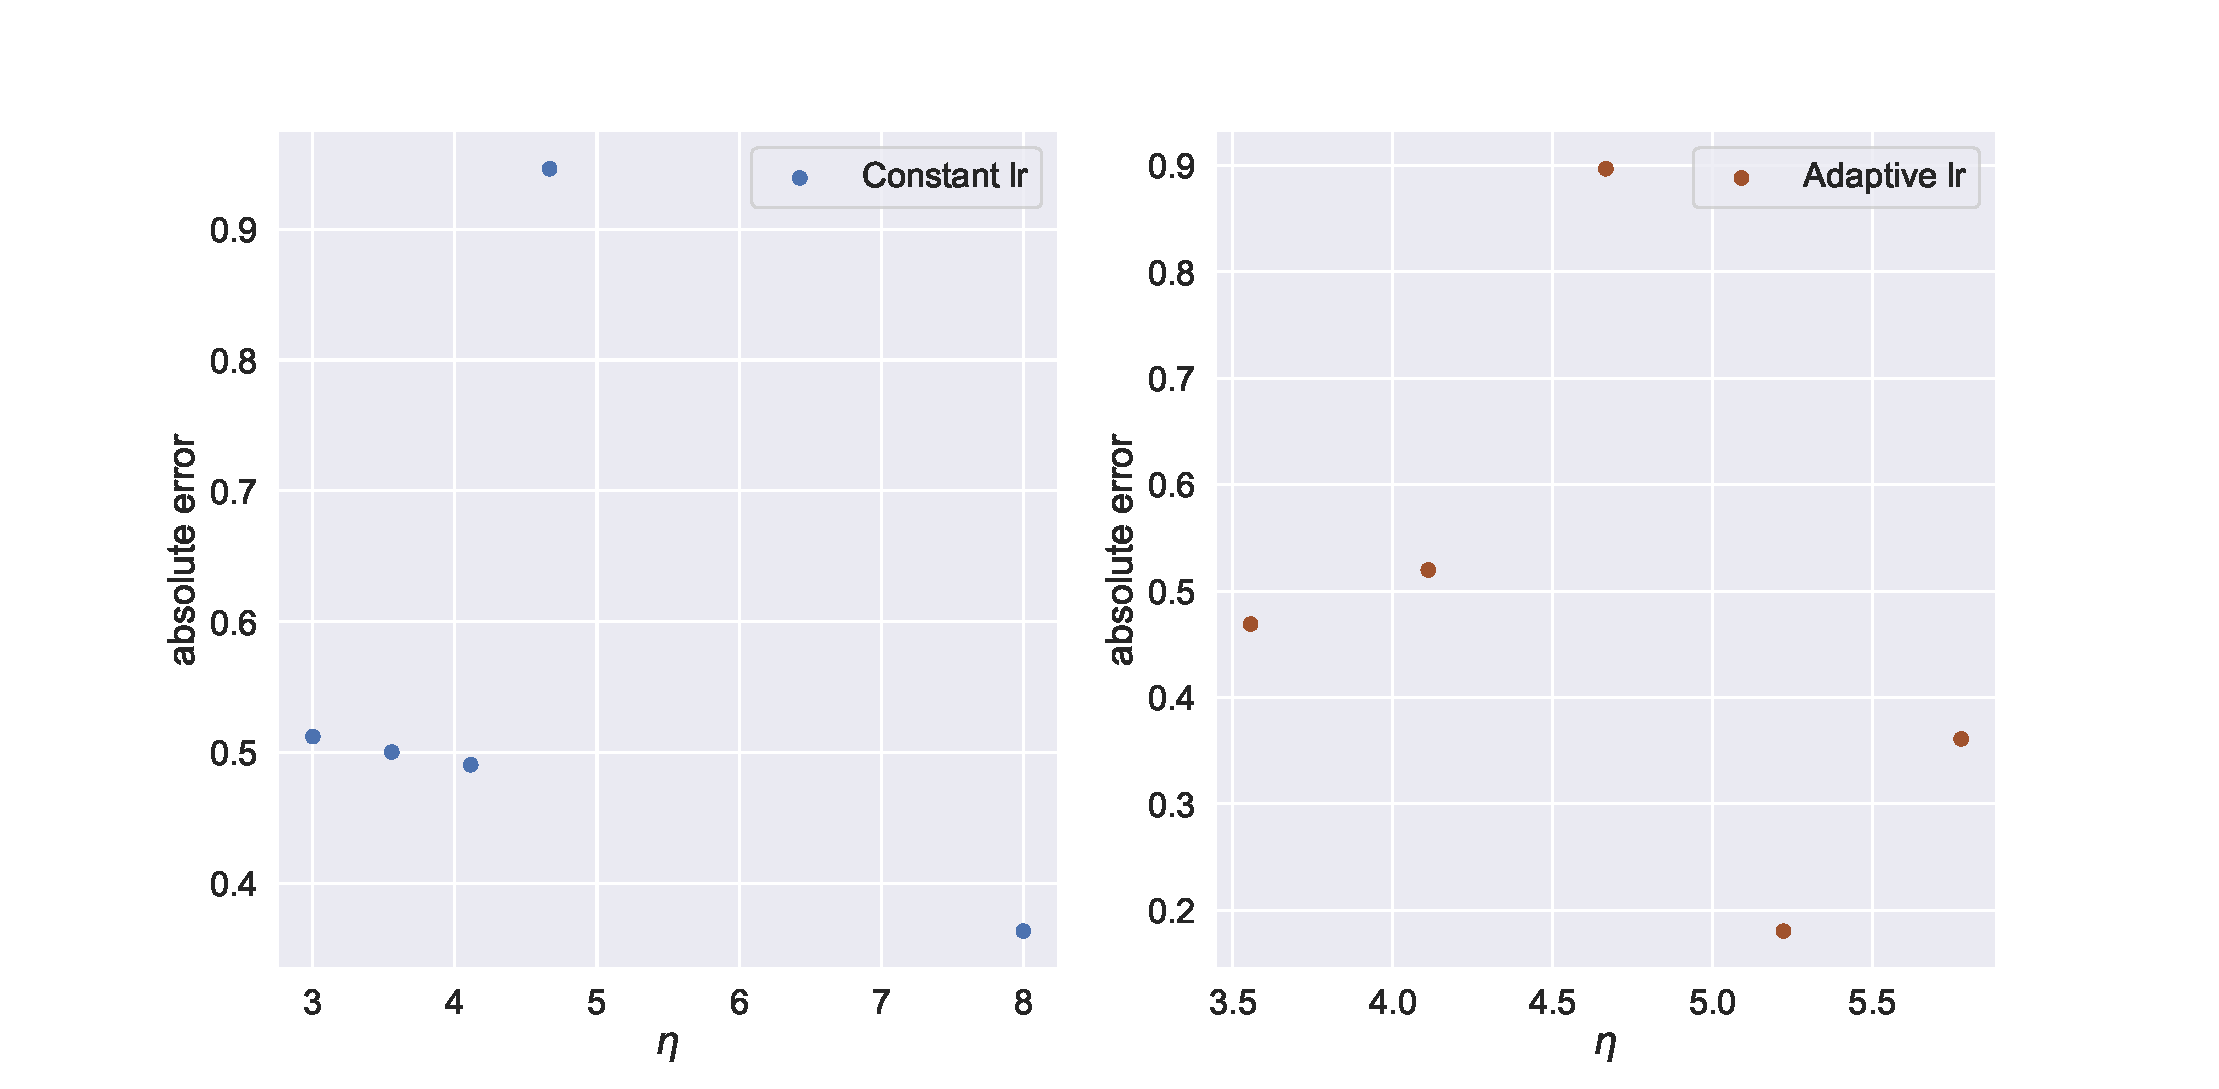
\includegraphics[width=0.5\textwidth]{Figures/Plots/Implementation Test/adapt_v_nop.pdf}
  \end{center}
  \caption{Comparison between no adaptive function, on the left, and with momentum, on the right, by checking the absolute error as a function of the learning rate. The 4-particle Lipkin model is used, with $\varepsilon = 1$, and interaction strengths $V=0.5$ and $W = 0$. Outliers has been removed to make the lower errors differentiable from each other.}\label{fig:adapt_imp_test}
\end{figure}

The training of the machine is very sensitive to changes in learning rate, and since we will use a range found suitable from the optimization section, \ref{sec:opt_lipkin}. Here we see that the momentum about halves the absolute error.


